\section{Durchführung}
\label{sec:Durchführung}
Der Versuch wird mit dem in Abbildung \ref{fig:Schaltung2} dargestellten Verstärker durchgeführt, der sich aus mehreren Modulen zusammensetzt (wie in der Abbildung zu sehen ist).
Zur Messung und Skizzierung der Spannungssignale wird ein digitales Oszilloskop verwendet.
Die Schaltung wird Schritt für Schritt nach Abbildung \ref{fig:Schaltung3} aufgebaut und nach jedem Bauelement wird das Signal betrachtet.
Der Ausgang \enquote{Oscillator} liefert das Referenzsignal und der Ausgang \enquote{Reference} das Messsignal.

Für die erste Messreihe soll ein Signal ohne Rauschen vermessen werden, der Noise Generator wird also auf \enquote{OFF} gestellt.
Ein sinusförmiges Messsignal von ungefähr 1 kHz und 10 mV wird, nachdem es verstärkt wurde, mit einer ebenfalls sinusförmigen Referenzspannung von gleicher Frequenz gemischt.
Das Signal, das danach den Detector verlässt, wird für 5 verschiedene Phasen mit Hilfe der Screenshotfunktion des Oszilloskops festgehalten.
Anschließend wird das Signal nach dem Tiefpass, also nach der Integration, in Abhängigkeit der Phasenverschiebung gemessen.
Es sollen 10 Messwerte genommen werden, die nach der Auswertung mit \eqref{eqn:gl3} verglichen werden sollen.
Die ganze Messung soll für ein verrauschtes Signal in der Größenordung der Messspannung wiederholt werden und beide Messreihen sollen miteinander verglichen werden.

Im letzten Versuchsteil soll eine Schaltung wie in Abbildung \ref{fig:Schaltung4} aufgebaut werden, um den Zusammenhang zwischen Lichtintensität der LED und dem Abstand $r$ zwischen LED und Photodiode zu untersuchen.
Das Blinken der Leuchtdiode soll dabei mit einer Rechtseckspannung und einer Frequenz zwischen 50 und 500 Hz moduliert werden.
Außerdem soll der maximale Abstand $r_{\text{max}}$ bestimmt werden, bei dem das Licht der LED noch nachweisbar ist.

\begin{figure}
  \centering
  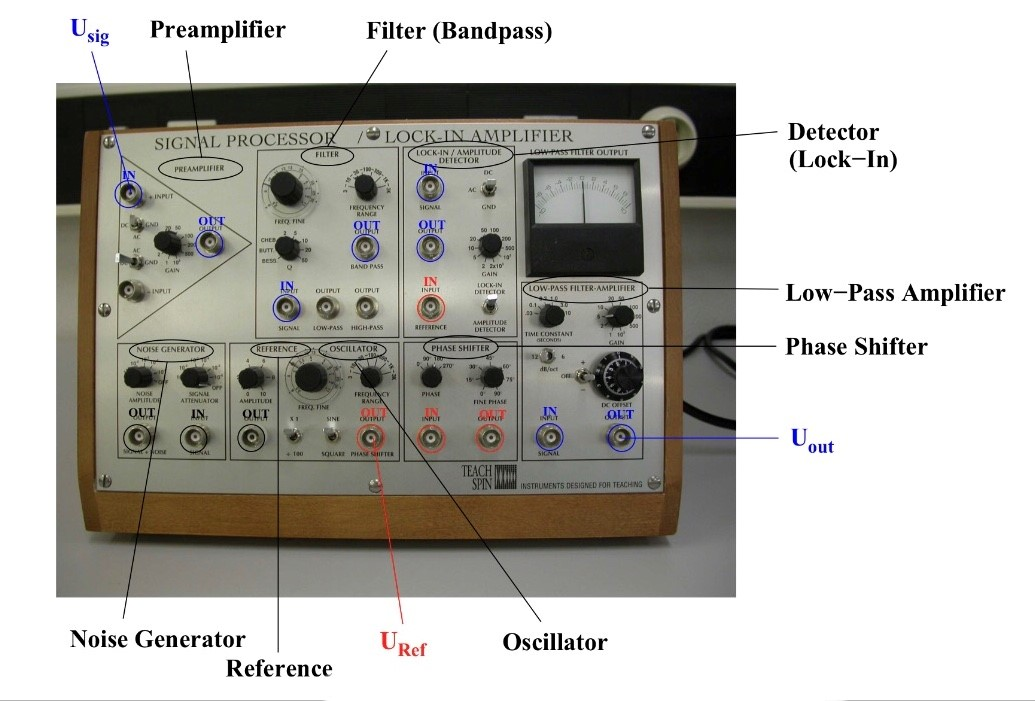
\includegraphics[width=\textwidth]{data/Schaltung2.jpg}
  \caption{Lock-In Verstärker \cite{V303}}
  \label{fig:Schaltung2}
\end{figure}

\begin{figure}
  \centering
  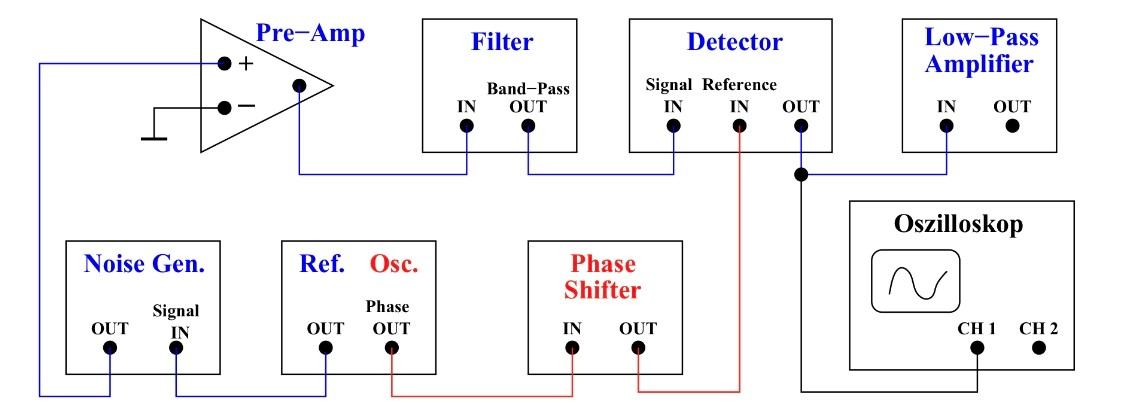
\includegraphics[width=\textwidth]{data/Schaltung3.jpg}
  \caption{Schaltplan eines Lock-In-Verstärkers \cite{V303}}
  \label{fig:Schaltung3}
\end{figure}

\begin{figure}
  \centering
  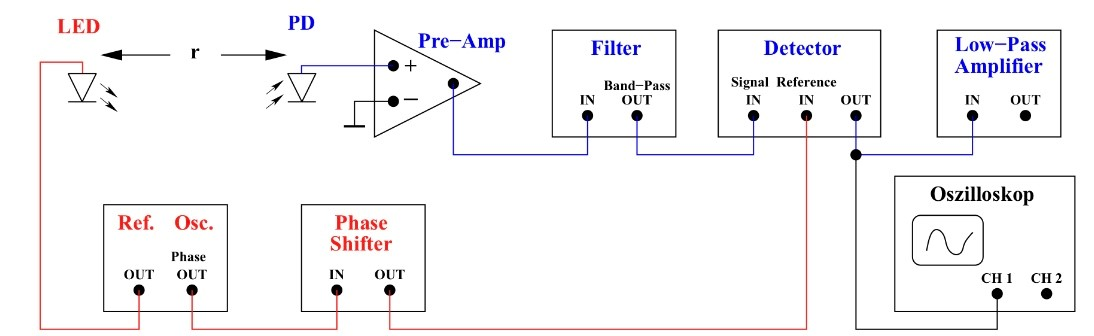
\includegraphics[width=\textwidth]{data/Schaltung4.jpg}
  \caption{Schaltplan eines Lock-In-Verstärkers \cite{V303}}
  \label{fig:Schaltung4}
\end{figure}
